% Compile from solution/: pdflatex solution.tex (twice for references).
\documentclass[10pt,a4paper]{article}
\usepackage[T1]{fontenc}
\usepackage[utf8]{inputenc}
\usepackage[margin=17mm,headheight=14pt]{geometry}
\usepackage{lmodern,microtype,graphicx,xcolor,booktabs,tabularx,array}
\usepackage{amsmath,tikz,fancyhdr}
\usetikzlibrary{arrows.meta,positioning}
\usepackage[colorlinks=true,urlcolor=teal,linkcolor=teal]{hyperref}
\definecolor{ink}{HTML}{20343B}
\definecolor{teal}{HTML}{007D78}
\definecolor{pale}{HTML}{EDF5F4}
\definecolor{rust}{HTML}{B84A27}
\renewcommand{\familydefault}{\sfdefault}
\color{ink}
\setlength{\parindent}{0pt}
\setlength{\parskip}{6pt}
\setlength{\tabcolsep}{5pt}
\renewcommand{\arraystretch}{1.15}
\pagestyle{fancy}
\fancyhf{}
\fancyhead[L]{\small Submitted to \textbf{TRESATA}\enspace /\enspace Finance AI take-home}
\fancyhead[R]{\small November 2026}
\fancyfoot[L]{\footnotesize Public and synthetic data only\enspace\textbullet\enspace Research prototype}
\fancyfoot[R]{\footnotesize\thepage\ / 4}
\renewcommand{\headrulewidth}{0.3pt}
\newcommand{\topic}[1]{\par\vspace{5pt}{\large\bfseries\color{teal}#1}\par\vspace{1pt}}
\newcommand{\smalltopic}[1]{\par\vspace{3pt}\textbf{#1}\par}
\newcommand{\code}[1]{{\footnotesize\nolinkurl{#1}}}
\newcommand{\captionline}[1]{{\footnotesize\color{ink!75}#1}\par}
\newcolumntype{Y}{>{\raggedright\arraybackslash}X}
\begin{document}
\thispagestyle{fancy}
{\fontsize{25}{28}\selectfont\bfseries Project brief}\par
{\large Turning company earnings announcements into usable research data}

\topic{1\enspace What this project does}
This project turns company earnings announcements into organised data for financial
research. These announcements describe a company's sales, profits and expectations
for the coming months. Reading them one by one is repetitive, especially when a
researcher wants to understand what is happening across many companies.

The workflow starts by selecting a group of companies and a reporting period. It
downloads their announcements, converts the documents into readable text, and uses
AI to identify revenue, earnings, future outlook and recurring business themes.
Each answer is stored with a short quote from the document. Code checks the numbers,
units and reporting periods, removes duplicate company records, and combines the
usable information into indicators for the group. This organised dataset is the
project's \textbf{knowledge base}.

\smalltopic{A simple example}
Suppose an announcement says, ``Revenue grew 10\% compared with last year.'' The AI
records the stated 10\% and its supporting quote. The checks look for that value in
the source and the relevant reporting period. If it passes, it can contribute to the
group's average revenue growth. If a figure is missing or doubtful, it is left out of
that calculation and flagged when review is needed.

The final output is a set of research indicators, including revenue growth, earnings
growth and the share of companies raising their outlook. Each includes
\textbf{coverage}: how many companies supplied usable information. The website shows
the workflow as connected nodes; clicking a node reveals its inputs and outputs.
Researchers can inspect the process and export the indicators for further analysis.

\smalltopic{Why I chose this problem}
The entire project idea came from my experience working as a quantitative researcher
intern at WorldQuant. I saw how financial information can be distilled and compressed
into inputs for alpha research---the search for signals that can inform investment
strategies. I wanted to build the data preparation workflow behind that kind of work,
using public documents and results that could be checked against their sources.

Manual comparison can mix up years, units or accounting definitions. Public filings
and free AI models made a prototype practical without buying a data feed; actual
time and cost savings still need measuring. An important detail was preserving table
columns: the right number from the wrong year is still a wrong answer. Earnings per
share (EPS) means profit per share; guidance means the company's future outlook.

\begin{center}
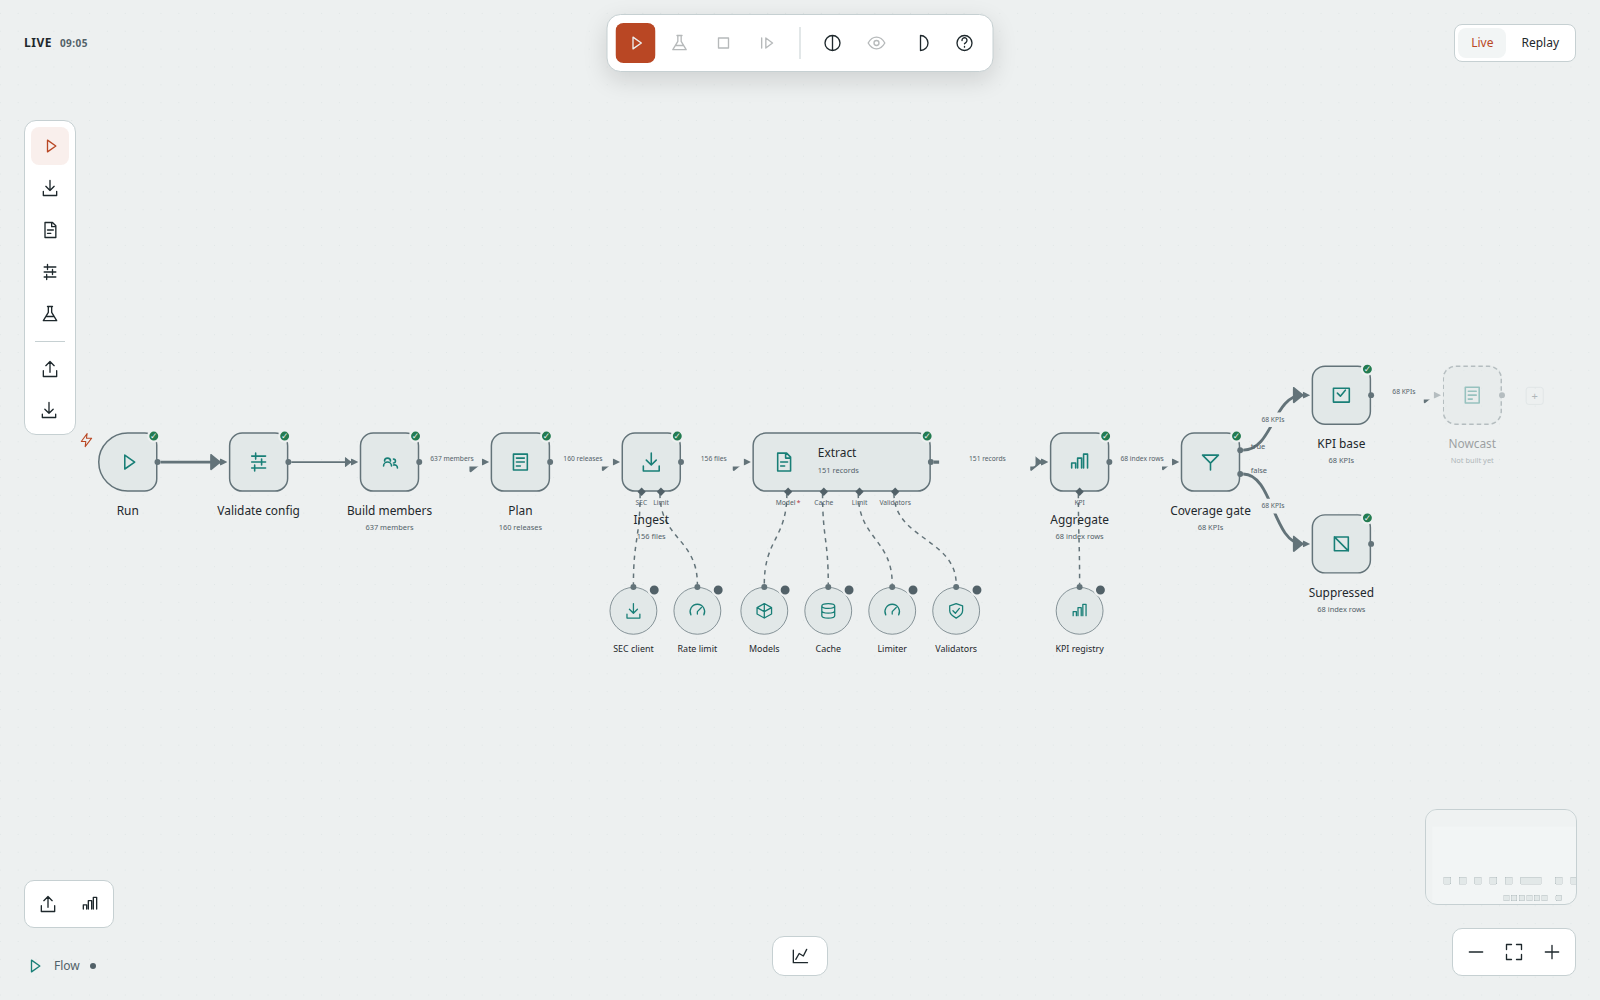
\includegraphics[width=\linewidth,trim=0 240 0 280,clip]{screenshots/01-workflow.png}
\end{center}
\captionline{The n8n-style workflow view. A failed coverage gate leads to suppression;
Nowcast is still planned.}

\topic{What this version covers}
The sources are earnings announcements filed with the SEC, the U.S. securities
regulator, as 8-K Item 2.02 releases and text exhibits. Historical S\&P 500 membership
determines eligibility. The default sample is 40 companies across four completed
calendar seasons, selected with seed 42 and fixed for the run. Sample coverage and
full-index coverage are reported separately.

This version stops at research indicators. It does not generate trading advice or
publish company-level results, and it uses no client data. RAPTOR retrieval, XBRL
enrichment and the Nowcast stage are planned. The indicators are sample-based proxies,
not official index earnings. Extending this to another country would require different
filing sources, identifiers, membership data and accounting/currency handling.

\newpage
\topic{2\enspace How the pipeline works}
\begin{center}
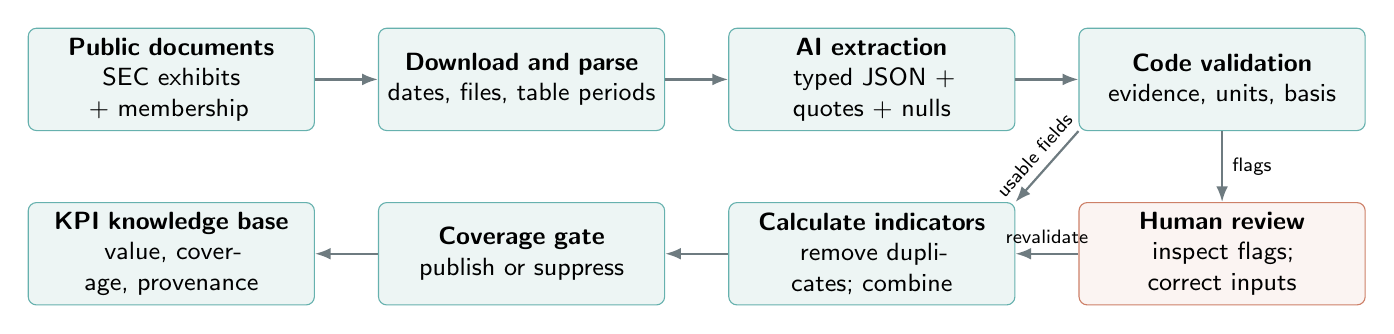
\begin{tikzpicture}[
  box/.style={draw=teal!60,fill=pale,rounded corners=3pt,align=center,
              text width=34mm,minimum height=13mm,font=\small},
  human/.style={box,draw=rust!70,fill=rust!6},
  arr/.style={-{Latex[length=2mm]},thick,draw=ink!65},
  node distance=5mm and 8mm]
  \node[box] (source) {\textbf{Public documents}\\SEC exhibits + membership};
  \node[box,right=of source] (parse) {\textbf{Download and parse}\\dates, files, table periods};
  \node[box,right=of parse] (ai) {\textbf{AI extraction}\\typed JSON + quotes + nulls};
  \node[box,right=of ai] (check) {\textbf{Code validation}\\evidence, units, basis};
  \node[human,below=9mm of check] (review) {\textbf{Human review}\\inspect flags; correct inputs};
  \node[box,left=of review] (calc) {\textbf{Calculate indicators}\\remove duplicates; combine};
  \node[box,left=of calc] (gate) {\textbf{Coverage gate}\\publish or suppress};
  \node[box,left=of gate] (out) {\textbf{KPI knowledge base}\\value, coverage, provenance};
  \draw[arr] (source)--(parse);
  \draw[arr] (parse)--(ai);
  \draw[arr] (ai)--(check);
  \draw[arr] (check)--node[right,font=\scriptsize]{flags}(review);
  \draw[arr] (check.south west)--node[above,sloped,font=\scriptsize]{usable fields}(calc.north east);
  \draw[arr] (review)--node[above,font=\scriptsize]{revalidate}(calc);
  \draw[arr] (calc)--(gate);
  \draw[arr] (gate)--(out);
\end{tikzpicture}
\end{center}
\captionline{Flagged results go to review. Fields that pass the checks can proceed
automatically; an analyst remains responsible for using the published results.}

\smalltopic{Extraction}
The parser turns web documents into text while keeping table labels and periods. The
AI model returns EPS, revenue, printed revenue growth, guidance, tone and themes in
JSON, a structured format that the code can read.
Each extracted value needs a supporting quote and a confidence value; missing or
ambiguous information should be null, with a reason. Normally this takes one call
per document. A second configured model can be tried if the first fails or has low
confidence. Caching, request budgets and saved receipts let interrupted work resume.
If a request's outcome is unknown, the run stops for attention before trying again.

AI is useful here because companies describe the same concepts in different ways,
especially guidance. A fixed template or set of regexes would need many exceptions.
The model's job is limited to interpreting and extracting the document. Code handles
the arithmetic and publication rules. I kept the workflow sequential: there is no
measured need yet for cooperating agents or a vector database. Documents are passed
within a configured context limit, which can omit useful passages in long releases.

\smalltopic{Checks and calculations}
Validators compare quotes and numbers against source text, including signs, scale,
period and accounting basis (standard/GAAP or company-adjusted). Flagged fields are withdrawn from their affected metrics;
blocking failures withdraw the record. Code collapses duplicate company-season records,
uses filing-date membership and excludes information published after each as-of date.
For comparable EPS bases, company growth is
\(g_i=(EPS_i-EPS_{i,\mathrm{prior}})/|EPS_{i,\mathrm{prior}}|\);
missing or zero prior values are excluded. Code limits the effect of extreme values
and applies the configured weights. The defaults require at least ten companies and ten usable observations
per metric. Missing analyst consensus leaves beat rate unavailable.

\smalltopic{Sources and changes}
The original documents are retained. KPI definitions and thresholds are stored in
configuration and code, and run manifests record fingerprints of the inputs, prompts
and settings. Exports include the metric, season, as-of date, units, observation counts,
status and hashes. An internal evidence view lets a reviewer trace a field to its source.
Changed inputs or settings require revalidation, and stale extractions are excluded.

\smalltopic{Risks and alternatives}
\begin{tabularx}{\linewidth}{@{}p{28mm}Y@{}}
\toprule
\textbf{Risk} & \textbf{Response and remaining limit}\\\midrule
Wrong answers & Source checks, nulls, review and suppression. Matching a quote does not prove its financial meaning; confidence is not calibrated accuracy.\\
Stale knowledge & Historical membership, as-of filtering and fingerprints. Membership reconstruction and fiscal/calendar alignment still need independent checks.\\
Confidentiality & Use public/synthetic inputs; keep credentials and evidence out of exports. Public text goes to the model provider; the workstation has no user login and needs a trusted environment.\\
Liability and bias & Label research proxies and coverage. A small, early-reporting cohort can misrepresent the index; no predictive or investment performance is established.\\
\bottomrule
\end{tabularx}
I would not ask one LLM call to produce the final index summary: checking every
calculation and omission would be difficult. Rules alone struggle with the prose,
while XBRL alone would leave out guidance and tone. Retrieval and XBRL are worth
revisiting once the remaining extraction errors are better understood.

\newpage
\topic{3\enspace Results}
The repo contains the Python pipeline, a CLI, a FastAPI backend and a React workflow
view. The website lets me inspect a step's inputs and outputs, review quality and cost,
replay results and export the KPIs. The saved runs show both progress and problems:

\begin{tabularx}{\linewidth}{@{}p{36mm}Y@{}}
\toprule
\textbf{Experiment} & \textbf{Observed result and interpretation}\\\midrule
10 public documents, two models & Saved bakeoff: ten companies across four seasons, same seed-42 sample. Both models parsed 10/10 replies; each produced nine nonempty extractions. Human-labelled accuracy is unavailable.\\
Lightning vs. Nano & Reported-EPS coverage: 80\% vs. 60\%; revenue: 90\% vs. 80\%; prior-year EPS: 10\% vs. 20\%. Median latency: 246.68\,s vs. 45.99\,s. These are saved observations, not current service guarantees.\\
Larger live run & Saved extraction manifest reports 151 saved results, five failures and 142 flagged outputs (including two empty). A parsed response is not a verified record; review remains a substantial burden.\\
500 synthetic releases & 125 invented companies over four seasons, using controlled model replies. All 400 planted errors (missing quote, wrong number, period or sign) were flagged; none of 100 clean cases were flagged. Aggregates exactly matched an independent pandas calculation. This offline check was rerun for the brief.\\
What this establishes & The synthetic test checks the safeguards using canned replies. The public-document runs exercise real models, but neither run establishes human-labelled accuracy, prompt-injection resistance or analyst time saved.\\
\bottomrule
\end{tabularx}

\begin{center}
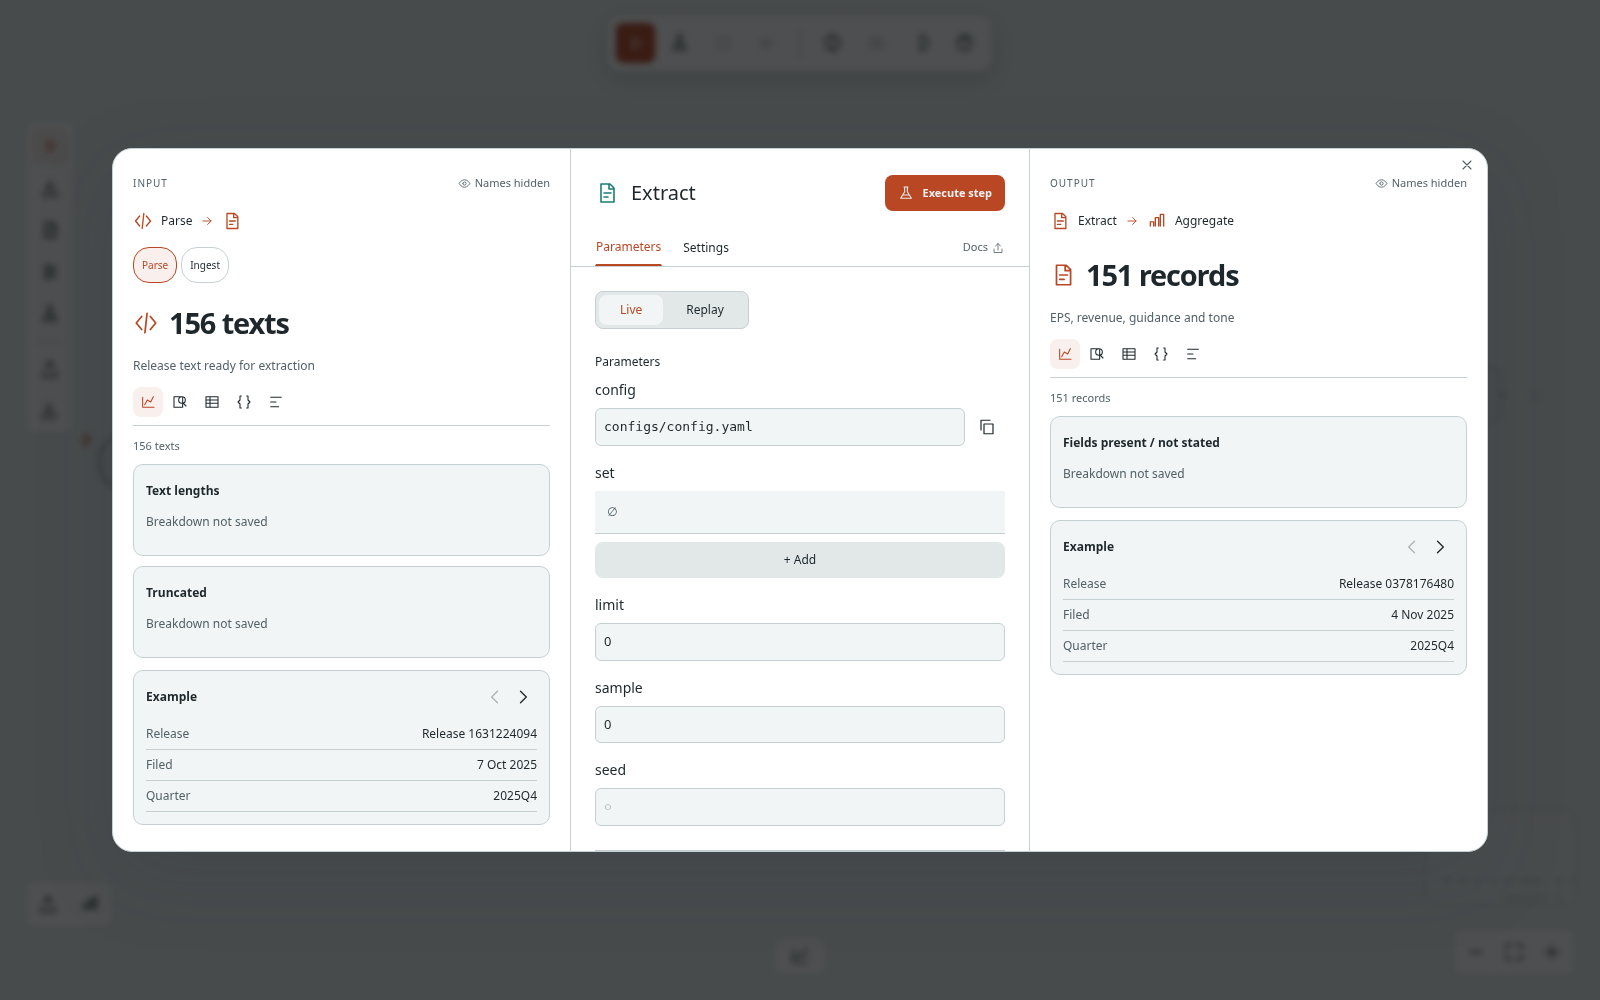
\includegraphics[width=\linewidth,height=64mm,keepaspectratio]{screenshots/03-inspector.png}
\end{center}
\captionline{Inspecting the extraction step: 156 input documents and 151 saved records.
\code{screenshots/02-quality.png} also shows the review-reason chart.}

\smalltopic{Where I would spend more time}
The 142 flagged outputs in the larger run are the main concern. Even a correctly copied
number may refer to a different period or accounting basis, and reviewing most of the
outputs could remove the benefit of automation. Calendar seasons can also misalign
with company fiscal periods, and tone remains subjective.

My next step would be to get an analyst to label a representative set of public
releases, then measure field-level precision, recall and minutes spent reviewing.
I would check the denominators and time alignment against a manual calculation and
compare the effort with using structured data directly. That would tell me whether
the pipeline is worth expanding. Testing whether these indicators help predict
anything is a separate step before building Nowcast.

\smalltopic{Run and inspect}
From the repository root: \texttt{./setup.sh bootstrap}, \texttt{./setup.sh init},
\texttt{./setup.sh demo}, then \texttt{./setup.sh website}; open
\url{http://localhost:8767}. Skip the API key for offline use. Public SEC downloads
require a contact-bearing user agent. Full instructions and model settings are in
\code{README.md} and \code{configs/config.yaml}.

\captionline{Evidence: \code{data/manifests/bakeoff.json};
\code{data/manifests/extract.manifest.json}; \code{src/nowcast/verification.py};
\code{tests/unit/test_validators.py}; \code{tests/unit/test_aggregate.py}.
Runtime evidence is local and excluded from the source archive.}

\newpage
\topic{Appendix\enspace What was added beyond AI}
The entire project idea was mine, based on my experience as a quantitative researcher
intern at WorldQuant. I used public and synthetic documents to explore it here; this
project contains no proprietary system or client data.

\smalltopic{Where AI helped}
I mainly used AI to improve the prompts: make the instructions clearer and make them
work across different documents. I also used it to build the n8n-style website,
debug the codebase and summarise scraped documents while exploring the data. The
summaries helped me understand the material; the metrics use the structured records
and their evidence checks. AI also helped edit this brief.

\smalltopic{Example prompts}
\begin{enumerate}
\setlength{\itemsep}{6pt}
\item \textbf{Making the prompt general:}\\
``This works for the example but feels too hardcoded. Can you make the prompt more
general so it works with other earnings releases too? Keep it clear, and don't fill
in values that aren't in the document.''
\item \textbf{Visualising the flow:}\\
``I want a website like n8n to visualise this project. Show how the data moves from
one node to the next, and let me click a node to see its inputs and outputs.''
\item \textbf{Debugging and understanding documents:}\\
``The number is in the document but the extraction is wrong. Help me trace where
this breaks. Please fix the underlying issue instead of adding a special case for
this file.''
\end{enumerate}

\smalltopic{What I rejected or corrected}
The main thing I had to push back on was hardcoding. A proposed fix could work for the
document in front of us but fail on a release with different wording or layout. I
corrected those ideas because the pipeline needs to work across companies. The tests
for periods, units, missing evidence and duplicate records help check that a fix
does more than make one example pass.

\smalltopic{What came from me}
The entire idea, the choice of problem and the overall data flow came from me.
They grew out of my internship experience working as a quantitative researcher at
WorldQuant. I decided how information should move from one major node to the next;
the website helped me visualise that design and inspect each step. AI helped me
implement, refine and debug the project.

\smalltopic{One thing to defend live, without AI}
I would be comfortable walking through the workflow without tools: selecting the
historical universe and panel, ingesting releases, parsing them, extracting and
checking fields, reviewing exceptions, and finally aggregating and exporting the
results. For each major node, I can explain what comes in, what goes out and what
happens when the step fails. That is the part of the project I would choose to defend live.
\end{document}
